\documentclass[border=1pt]{standalone}
\usepackage{tikz}

\begin{document}
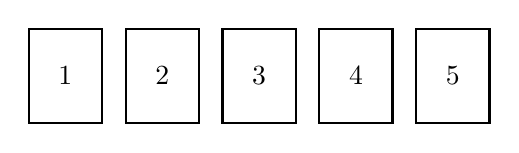
\begin{tikzpicture}
    \pgfmathsetmacro{\xa}{.93}
    \pgfmathsetmacro{\xb}{.3}
    \pgfmathsetmacro{\xab}{\xa+\xb}
    \pgfmathsetmacro{\ya}{1.2}
    \foreach \n in {1,...,5} {
        \draw[thick] ({(\n-1)*\xab},0) rectangle +(\xa,\ya);
        \node at ({(\n-1)*\xab+0.5*\xa},0.5*\ya) { \n };
    }
\end{tikzpicture}
\end{document}
